%part
% 2024-02-16.tex chapter
\chapter[\textit{Introduction} by Lyle Dowling]{\center{INTRODUCTION \\[1ex]\large{by ARNOLD SHAW and LYLE DOWLING}\\Co-editors \textit{Schillinger System of Musical Composition}}}
The Schillinger system is a synthesis of musical theory and the most recent
discoveries of modern physics, physchology, and mathematics. Historically, it represents the first successful effor tto classify scientifically the resources of our musical system. In view of the highly original character of Schillinger's approach, a brief description of his methodology and underlying ideas seems desirable.\footnote{The material in this Introduction is based in part on lectures delivered by Arnold Shaw at the Julliard School of Music during the summer of 1945.}
\section{Music and Science}
Efforts to establish Musical theory on a scientif basis date back to
antuiquity. Among the Greeks, Pythagoras and his followers investigated the
mathematical ratios underlyiing harmonic intervals. Down the ages the
fabrication of musical instruments and the theory of instrumentation have been
correlated with developments in physics and mathematics. Within the past 200
years, two of the greatest musical theorists based their work on scientific
data. In Jean-Philippe Rameau's \textit{Treatise on Harmony} (1722), we have
the beginnings of a school of thought, recently given new impetus, that makes
acoustics the foundation of musical theory. In \textit{Sensations of Tone}
(1863) Helmholtz developed his theories on the basis of the findings of
physiology and psychology. Zarlino, Kircher, Tanaeiev and others have evolved
theories employing data of the various sciences. In \textit{The Craft of
Musical Composition}, Paul Hindemith, commenting on the pleasure derived from
hearing vibration-combinations in simple ratios, writes: \say{This basic fact
of our hearing process reveals to us how closely related are number and beauty,
mathematics and art}.

Despite this history, the idea of mixing music with mathematics is a
disquieting one to some. Since music is generally portrayed as the most
evanescent of the arts, to wed it to the most exacting and the most rigid of
the sciences seems to produce an ill-concieved union. In part the feeling of
uneasiness may stem also from an unconscious desire on the part off some
composers to keep their craft in the realm of the cabalistic mysteries.

From the historical point of view, the clash between the arts and sciences is
of comparatively recent origin---for us, largely the result of the romantic
movement. We are heirs of the tradition that swept across the Europe and the
United States toward the end of the eighteenth century and that revived Plato's
view of the artist as an inspired madman. As a reulst both critical and lay
musical circles tend to exalt inspiration, genius and intuition over knowledge
of resources, mastery of technique, craftsmanship, etc. Viewed practically, the
dichotomy between learning and genius---between science and art---is not merely
a product of romanticism. It has also been the result of the limitations of
musical theory and pedagogy\footnote{One of our most enlightened contemporary
theorists and composers, Walter Piston of Harvard University, describes musical
theory in his book on \textit{Harmony} as follows: \say{If we reflect that
theory must follow practice, rarely preceding it except by chance, we must
realize that musical theory is not a set of directions for composing music. It
is rather the collected and systematized deductions gathered by observing the
practice of composers over a long time, and it attempts to set forth what is or
has been the common practice. It tells not how music will be written in the
future, but how music has been written in the past}}. If you cannot define and
explain certain aspects of musical composition you fall back of necessity, on
that vague and indefinable thing called \say{genius} or \say{inspiration}.
Schillinger's own experience as a student at the St. Petersburg
Conservatory\footnote{Schillinger (1895-1943) entered the St. Petersburg
Imperial Conservatory in 1914 and was graduated in 1918. A biographical sketch
is included at the end of Volume II of the present work.} led him to embark on
the investigation that yielded, after twenty five years of work, the theory now
known as the Schillinger System.

Schillinger's voyage of intellectual discovery began in 1914 while he was a
student atht eh St. Petersburg Conservatory. It continued during a period of
ten years (1918-1928) while he held various teaching posts in his native
Russia. On coming to the United States in 1928, it took on new impetus as a
resultof ohis collaborating with Leon Theremin on electro-magnetic musical
experiments and inventions. From 1932 on, when much of the system had taken
form, Schillinger had opportunities to test it at various American schools and
colleges. He was either a lecturer or an inst4ructor at the David Berend School
of Music, the Florence Cane School of Art, the New School for Social Research,
and New York University. The reaches of his theory, embracing as it did
mathematics, music and the spatial arts, were afforded varied expression at
Columbia :University where he gave courses or lectures in three departments:
the Mathematics, Fine Arts and Music departments of Teachers College. When
Schillinger was convinced of the practical nature of his discoveries, he turned
also to private instruction. So successful were his students as composers and
arrangers for radio, the motion pictures and the theatre that Schillinger
attracted to his studio many of America's best known musicians.\footnote{A
partial list of Schillinger students would include: George Gershwin, who
studied for more than four years; Oscar Levant, Glenn Miller, Benny Goodman,
Paul Lavalle, Nathan Van Cleave, Lyn Murray, Charles Previn, Will Bradly, Jesse
Crawford, Carmine Coppola, Lennie Hayton, Joseph Lilley, Jeff Alexander,
Franklyn Marks, Jack Miller, Edward Powell, Alvino Rey, Ted Royal, Frank
Skinner, Herbert Spencer, Paul Sterrett, Leith Stevens, Mme Koshetz, Lazar
Weiner; also Dr. Myron Schaffer, formerly head of the music department of the
University of Panama; and Edwin Gerschefski, Dean of the School of Music of
Converse College.} By the time of his sudden death in March in 1943, Schillinger regarded his theories as sufficiently formulated to have incorporated them in two significant works: \textit{Mathematical Basis of the Arts} and the present publication.

\section{Mathematics of Voice Leading} A valuable clue to Schillinger's
approach to music is offered by him in his introduction to Book V,
\textit{Special Theory of Harmony}. \say{The main defect of existing theories
of harmonies}, he writes, \say{is in the use of the \textit{descriptive
method}. Each case is analyzed apart from all other cases and without yielding
any general underlying principles. But the mathematical treatment of the
subject discloses general properties of the positions and movements of the
voices in terms of the transformation of chordal functions.} Schillinger
thereupon proceeds on the assumption that any chord is an assemblage of
pitch-units, or to use mathematical terminology, a group of conjugate elements.
In three-part structures $(S = 3p)$, the voices or functions may be designated
as a, b, and c, or 1, 3, 5.

\begin{center}
	\begin{lilypond}[notime,fragment,staffsize=20]
		\new Staff \with {
			\consists Balloon_engraver
			\override BalloonText.annotation-balloon = ##f
			\override BalloonText.annotation-line = ##f
			\override Clef.space-alist.first-note = #'(minimum-fixed-space . 10.0)
		}
		{
			\relative c' {
				\balloonLengthOn
				\override Score.SpacingSpanner.spacing-increment = #3
				\override BalloonText.layer = #-2
				\override Staff.StaffSymbol.layer = #-3
				\override BalloonText.whiteout = ##t
				<
				e-\balloonText #'(0.1 . 0) \markup{"3"}
				-\balloonText #'(-1.5 . 0) \markup{"b"}
				g-\balloonText #'(1.3 . 0) \markup{"5"}
				-\balloonText #'(-0.5 . 0) \markup{"c"}
				c-\balloonText #'(0.1 . 0) \markup{"1"}
				-\balloonText #'(-1.5 . 0) \markup{"a"}
				>2
				<
				g,-\balloonText #'(0.3 . 0) \markup{"5"}
				-\balloonText #'(-0.5 . 0) \markup{"c"}
				e'-\balloonText #'(0.3 . 0) \markup{"3"} 
				-\balloonText #'(-0.5 . 0) \markup{"b"}
				c'-\balloonText #'(0.3 . 0) \markup{"1"} 
				-\balloonText #'(-0.5 . 0) \markup{"a"}
				>
			}
		}
	\end{lilypond}
\end{center}

It is to be observed that clockwise structures (reading downwards) are traditionally known as \textit{open} positions,


\begin{center}
	$\left[
		\begin{tabular}{c}
			1\\
			3\\
			5
		\end{tabular}
	\right]$
	$\left[
		\begin{tabular}{c}
			3\\
			5\\
			1
		\end{tabular}
	\right]$
	$\left[
		\begin{tabular}{c}
			5\\
			1\\
			3
		\end{tabular}
	\right]$
	\raisebox{-4.3ex}{
		\begin{lilypond}[notime,fragment,staffsize=20]
			\new Staff \with {
				\consists Balloon_engraver
				\override BalloonText.annotation-balloon = ##f
				\override BalloonText.annotation-line = ##f
				\override Clef.space-alist.first-note = #'(minimum-fixed-space . 7.0)
			}
			\relative c' {
				\balloonLengthOn
				\override Score.SpacingSpanner.spacing-increment = #2.2
				\override BalloonText.layer = #-2
				\override Staff.StaffSymbol.layer = #-3
				\override BalloonText.whiteout = ##t
				<
				f-\balloonText #'(-1 . 0) \markup{"1"} 
				c'-\balloonText #'(-1 . 0) \markup{"5"}
				a'-\balloonText #'(-1 . 0) \markup{"3"}
				>2
				<
				c-\balloonText #'(-1 . 0) \markup{"5"} 
				a'-\balloonText #'(-1 . 0) \markup{"3"} 
				f'-\balloonText #'(-1 . 0) \markup{"1"} 
				>
				<
				a'-\balloonText #'(-1 . 0) \markup{"3"} 
				f'-\balloonText #'(-1 . 0) \markup{"1"} 
				c'-\balloonText #'(-1 . 0) \markup{"5"} 
				>
			}
		\end{lilypond}
	}
\end{center}
and counterclockwise structures (reading downwards) as \textit{close}.


\begin{center}
	$\left[
		\begin{tabular}{c}
			1\\
			5\\
			3
		\end{tabular}
	\right]$
	$\left[
		\begin{tabular}{c}
			5\\
			3\\
			1
		\end{tabular}
	\right]$
	$\left[
		\begin{tabular}{c}
			3\\
			1\\
			5
		\end{tabular}
	\right]$
	\raisebox{-3.7ex}{
		\begin{lilypond}[notime,fragment,staffsize=20]
			\new Staff \with {
				\consists Balloon_engraver
				\override BalloonText.annotation-balloon = ##f
				\override BalloonText.annotation-line = ##f
				\override Clef.space-alist.first-note = #'(minimum-fixed-space . 9.0)
			}
			\relative c' {
				\balloonLengthOn
				\override Score.SpacingSpanner.spacing-increment = #2.5
				\override BalloonText.layer = #-2
				\override Staff.StaffSymbol.layer = #-3
				\override BalloonText.whiteout = ##t
				<
				f-\balloonText #'(-0.5 . 0) \markup{"1"} 
				a-\balloonText #'(-2 . 0) \markup{"3"}
				c-\balloonText #'(-0.5 . 0) \markup{"5"}
				>2
				<
				a-\balloonText #'(-0.5 . 0) \markup{"3"} 
				c-\balloonText #'(-2 . 0) \markup{"5"} 
				f-\balloonText #'(-0.5 . 0) \markup{"1"} 
				>
				<
				c,-\balloonText #'(-0.5 . 0) \markup{"5"} 
				f-\balloonText #'(-2 . 0) \markup{"1"} 
				a-\balloonText #'(-0.5 . 0) \markup{"3"} 
				>
			}
		\end{lilypond}
	}
\end{center}

Insofar as voice-leading is concerned, these voices behave, Schillinger
demonstrates, not through any musical specifications but through
\textit{general forms of transformation}. They move in a
clockwise(\raisebox{-1ex}{\includesvg[width=0.5cm]{../asset_2}}) direction, a counterclockwise(\raisebox{-1ex}{\includesvg[width=0.5cm]{../asset_1}}) direction, or
in some variation of these when one voice is constant.
\nopagebreak

\begin{center}
	\begin{tabular}{ c | c | c | c }
		&
		\textit{Clockwise} (\raisebox{-1ex}{\includesvg[width=0.5cm]{../asset_2}}) \hspace{2mm} \raisebox{-2.5ex}{\includesvg[width=1cm]{../asset_4.svg}} \hspace{2mm}&
		\textit{Counterclockwise} (\raisebox{-1ex}{\includesvg[width=0.5cm]{../asset_1}}) \hspace{2mm} \raisebox{-2.5ex}{\includesvg[width=1cm]{../asset_5.svg}} &
		\textit{Constant 3} \\
																				   & & & \\
		\hline
		&
		\begin{tabular}{l r}
			\textit{First chord} &
			\textit{Next chord}
		\end{tabular} &
		\begin{tabular}{l r}
			\textit{First chord} &
			\textit{Next chord}
		\end{tabular} &
		\begin{tabular}{l r}
			\textit{First chord} &
			\textit{Next chord}
		\end{tabular} \\
		\hline
		\multirow[c]{3}{*}[-1mm]{\rotatebox{90}{Voices}} &
		      \begin{tabular}{l c c c r}
			      1 & & \rightarrow & & 3
		      \end{tabular}
		      &
		      \begin{tabular}{l c c c r}
			      1 & & \rightarrow & & 5
		      \end{tabular}
		      &
		      \begin{tabular}{l c c c r}
			      1 & & \rightarrow & & 5
		      \end{tabular} \\
		      &
		      \begin{tabular}{l c c c r}
			      3 & & \rightarrow & & 5
		      \end{tabular}
		      &
		      \begin{tabular}{l c c c r}
			      3 & & \rightarrow & & 1
		      \end{tabular}
		      &
		      \begin{tabular}{l c c c r}
			      3 & & \rightarrow & & 3
		      \end{tabular} \\
		      & 
		      \begin{tabular}{l c c c r}
			      5 & & \rightarrow & & 1
		      \end{tabular}
		      &
		      \begin{tabular}{l c c c r}
			      5 & & \rightarrow & & 3
		      \end{tabular}
		      &
		      \begin{tabular}{l c c c r}
			      5 & & \rightarrow & & 1
		      \end{tabular} \\
\end{tabular}
\end{center}

\vspace{10mm}

Without developing the theory, which is presented in detail in Book V, but
simply to illustrate---suppose we have a triad on C followed by a triad on F.
From a mathematical standpoint---and we soon discover, also from a musical
standpoint, depending on sequence and the effect desired---here is what may
happen according to the general forms of transformation:
% \nobreak

\vspace{10mm}

\begin{lilypond}[notime,fragment,staffsize=14.5]
	\new Score \with {
		\consists Balloon_engraver
		\override BalloonText.annotation-balloon = ##f
		\override BalloonText.annotation-line = ##f
		\override Clef.space-alist.first-note = #'(minimum-fixed-space . 8.0)
	}
	{
		\new PianoStaff <<
		\new Dynamics = "rotation" {
			\repeat unfold 3 {
				s1^\markup {\halign #-3 \epsfile #X #3 #"../schillinger-clockwise-001.eps"}
				s^\markup {\halign #-3 \epsfile #X #3 #"../schillinger-counterclockwise-001.eps"}
			}
		}
		\new Staff {
			\balloonLengthOn
			\override Score.SpacingSpanner.spacing-increment = #3
			\override BalloonText.layer = #-2
			\override Staff.StaffSymbol.layer = #-3
			\override BalloonText.whiteout = ##t
			\relative c' {
				<
					c-\balloonText #'(-0.5 . 0) \markup{"1"}
					e-\balloonText #'(-2 . 0) \markup{"3"}
					g-\balloonText #'(-0.5 . 0) \markup{"5"}
				>2
				<
					a-\balloonText #'(-0.5 . 0) \markup{"3"}
					c-\balloonText #'(-2 . 0) \markup{"5"}
					f-\balloonText #'(-0.5 . 0) \markup{"1"}
				> % bar 1
				<
					c-\balloonText #'(-0.5 . 0) \markup{"1"}
					e-\balloonText #'(-2 . 0) \markup{"3"}
					g-\balloonText #'(-0.5 . 0) \markup{"5"}
				>
				<
					c-\balloonText #'(-0.5 . 0) \markup{"5"}
					f-\balloonText #'(-2 . 0) \markup{"1"}
					a-\balloonText #'(-0.5 . 0) \markup{"3"}
				> % bar 2
				<
					c-\balloonText #'(-0.5 . 0) \markup{"1"}
					g'-\balloonText #'(-0.5 . 0) \markup{"5"}
					e'-\balloonText #'(-0.5 . 0) \markup{"3"}
				>
				<
					a-\balloonText #'(-0.5 . 0) \markup{"3"}
					f'-\balloonText #'(-0.5 . 0) \markup{"1"}
					c'-\balloonText #'(-0.5 . 0) \markup{"5"}
				> % bar 3
				<
					c-\balloonText #'(-0.5 . 0) \markup{"1"}
					g'-\balloonText #'(-0.5 . 0) \markup{"5"}
					e'-\balloonText #'(-0.5 . 0) \markup{"3"}
				>
				<
					c-\balloonText #'(-0.5 . 0) \markup{"5"}
					a'-\balloonText #'(-0.5 . 0) \markup{"3"}
					f'-\balloonText #'(-0.5 . 0) \markup{"1"}
				> % bar 4
				<
					g'-\balloonText #'(-0.5 . 0) \markup{"5"}
					c-\balloonText #'(-2 . 0) \markup{"1"}
					e-\balloonText #'(-0.5 . 0) \markup{"3"}
				>
				<
					f-\balloonText #'(-0.5 . 0) \markup{"1"}
					a-\balloonText #'(-2 . 0) \markup{"3"}
					c-\balloonText #'(-0.5 . 0) \markup{"5"}
				> % bar 5
				<
					g-\balloonText #'(-0.5 . 0) \markup{"5"}
					c-\balloonText #'(-2 . 0) \markup{"1"}
					e-\balloonText #'(-0.5 . 0) \markup{"3"}
				>
				<
					a-\balloonText #'(-0.5 . 0) \markup{"3"}
					c-\balloonText #'(-2 . 0) \markup{"5"}
					f-\balloonText #'(-0.5 . 0) \markup{"1"}
				> % bar 6
			}
		}
		\new Staff {
			\clef "bass"
			\repeat unfold 3 {
				\relative c {
					c f
					\bar "|"
					c f
					\bar"||"
				}
			}
		}
		>>
	}
\end{lilypond}

\vspace{10mm}

\begin{lilypond}[notime,fragment,staffsize=14.5]
	\new Score \with {
		\consists Balloon_engraver
		\override BalloonText.annotation-balloon = ##f
		\override BalloonText.annotation-line = ##f
		\override Clef.space-alist.first-note = #'(minimum-fixed-space . 8.0)
	}
	{
		\new PianoStaff <<
		\new Dynamics = "rotation" {
			\repeat unfold 3 {
				s1^\markup {\halign #-2.5 \epsfile #X #3 #"../schillinger-clockwise-001.eps"}
				s^\markup {\halign #-2.5 \epsfile #X #3 #"../schillinger-counterclockwise-001.eps"}
			}
		}
		\new Staff {
			\balloonLengthOn
			\override Score.SpacingSpanner.spacing-increment = #3
			\override BalloonText.layer = #-2
			\override Staff.StaffSymbol.layer = #-3
			\override BalloonText.whiteout = ##t
			\relative c'' {
				<
					g-\balloonText #'(-0.5 . 0) \markup{"5"}
					e'-\balloonText #'(-0.5 . 0) \markup{"3"}
					c'-\balloonText #'(-0.5 . 0) \markup{"1"}
				>2
				<
					f-\balloonText #'(-0.5 . 0) \markup{"1"}
					c'-\balloonText #'(-0.5 . 0) \markup{"5"}
					a'-\balloonText #'(-0.5 . 0) \markup{"3"}
				> % bar 1
				<
					g-\balloonText #'(-0.5 . 0) \markup{"5"}
					e'-\balloonText #'(-0.5 . 0) \markup{"3"}
					c'-\balloonText #'(-0.5 . 0) \markup{"1"}
				>
				<
					a-\balloonText #'(-0.5 . 0) \markup{"3"}
					f'-\balloonText #'(-0.5 . 0) \markup{"1"}
					c'-\balloonText #'(-0.5 . 0) \markup{"5"}
				> % bar 2
				<
					e-\balloonText #'(-0.5 . 0) \markup{"3"}
					g-\balloonText #'(-2 . 0) \markup{"5"}
					c-\balloonText #'(-0.5 . 0) \markup{"1"}
				>
				<
					c-\balloonText #'(-0.5 . 0) \markup{"5"}
					f-\balloonText #'(-2 . 0) \markup{"1"}
					a-\balloonText #'(-0.5 . 0) \markup{"3"}
				> % bar 3
				<
					e-\balloonText #'(-0.5 . 0) \markup{"3"}
					g-\balloonText #'(-2 . 0) \markup{"5"}
					c-\balloonText #'(-0.5 . 0) \markup{"1"}
				>
				<
					f-\balloonText #'(-0.5 . 0) \markup{"1"}
					a-\balloonText #'(-2 . 0) \markup{"3"}
					c-\balloonText #'(-0.5 . 0) \markup{"5"}
				> % bar 4
				<
					e-\balloonText #'(-0.5 . 0) \markup{"3"}
					c'-\balloonText #'(-0.5 . 0) \markup{"1"}
					g'-\balloonText #'(-0.5 . 0) \markup{"5"}
				>
				<
					c-\balloonText #'(-0.5 . 0) \markup{"5"}
					a'-\balloonText #'(-0.5 . 0) \markup{"3"}
					f'-\balloonText #'(-0.5 . 0) \markup{"1"}
				> % bar 5
				<
					e-\balloonText #'(-0.5 . 0) \markup{"3"}
					c'-\balloonText #'(-2 . 0) \markup{"1"}
					g'-\balloonText #'(-0.5 . 0) \markup{"5"}
				>
				<
					f-\balloonText #'(-0.5 . 0) \markup{"1"}
					c'-\balloonText #'(-2 . 0) \markup{"5"}
					a'-\balloonText #'(-0.5 . 0) \markup{"3"}
				> % bar 6
			}
		}
		\new Staff {
			\clef "bass"
			\repeat unfold 3 {
				\relative c {
					c f
					\bar "|"
					c f
					\bar"||"
				}
			}
		}
		>>
	}
\end{lilypond}

\vspace{10mm}
\hspace{51mm}\includesvg[width=6cm]{../cc_n_c}
\vspace{2mm} \\

Additional possibilities may be developed if one of the voices is constant, i.e., 3 \rightarrow\ 3, 1 \rightarrow\ 1, or 5 \rightarrow\ 5.

\section{Schillinger's Major Aims}

On the basis of these illustrations, certain inferences may be drawn concerning Schillinger's aims. First, that he is concerned with discovering \textit{general underlying principles} of the behavior of tonal phenomena. Unlike most theoreticians who have preceded him, his generalizations are not based on the practices of selected composers, or selected schools of music. He is not interested in dogmatic rules, based on the achievements of given composers, or in countless exceptions to such rules, coined to explain practices characteristic of other composers. Schillinger is interested in generalizations based on the properties of tonal materials themselves and on the possible combinatsion, permutations and structural relatsions of such materials.

Secondly, he is interested in uncovering and classifying \textit{all of the available resources of our tonal system}. To be sure, this is a gargantuan task. Yet in a sense, it has been the expressed or unexpressed goal of all musical theorists. Somne approached it by way of musical usage. Along this road, success was attainable provided analysis was not limited to given composers, given schools, or given musical civilizations---and then this procedure could not encompass the future. Some theroists approached the goal of exhaustiveness by way of tonal materials themselves, which could chart the future. Unfortunately, no theorist prior to Schillinger adopted a methodology of sufficient scope to achieve the desired result. This is another way of saying that no theorist adopted the method of mathematics.

For it must be evident that mathematics as the general science of number, sequence, combination and structure presents the necessary and most practical tool for achieving complete classification.

Beyond these two purposes, Schillinger set himself a third and larger goal, but a necessary corollary of the first two. From the standpoint of science, analysis implies synthesis. Success in reducing a process or a substance to its component elements implies the ability to reconstruct the object or process through synthesizing such elements. The ultimate in science is not attained when we discover that atomic energy is the source of the sun's power. We achieve the ultimate when we can reproduce such power in the atomic bomb. From Schillinger's standpoint, therefore, scientific analysis of the tonal art implied scientific synthesis as a corollary. If one could take a composition and reduce it through computation to its component elements, then mastery of the process implied and ability to compose through computation. To be sure, this is the juncture at which Schillinger would run into conflict most sharply with tradition. Insofar as he succeeded in elaborating a method of composing through the preselection and synthesis of component tonal elements, he could expect strong opposition from certain quarters. But this was unavoidable.

From a scientific standpoint Schillinger's achievement of his first two aims [1) generalizing underlying princibles and 2) classifying tonal resources] is demonstrated by his success in applying the m4ethodology to composition itself. Earlier scientific approaches to musical theory were partial in charactyer. Their generalizations were applicable to given aspects, not to the art of composition as a whole. In Schillinger we encounter for the first time a comprehensive application of scientific method to all components of the tonal art, to problems of rhythm, melody, harmony, counterpoint, instrumentation, etc., and to the fundamental problem of all---composition itself. The individual techniques evolved in the different books---(1) temporal organization (Book I); (2) development of pitch-scales (Book II); (3) composition of melody (Books III and IV); (4) formation of chord structures and progressions (Books V and IX); (5) melodization of harmony (Book VII)---these individual techniques are all integrated in Book XI, \textit{Theory of Composition}. As Schillinger phrases it, his complete method involves \say{the prefabrication and the essembly of components according to a preconceived design of the whole.}

\section{Tools and Concepts}

It is to be noted that the tools of analysis employed by Schillinger were available to musical theroists long before he used them. The graph method, a commonplace in our daily stock reports, is almost three hundred years old. Trigonometry and algebra are of ancient origin. The jarriage of music and mathematics was not achieved because the basixc concepts to make it possible were lacking. These concepts are of comapratively recent origin although the tools are not. These concepts stem from the findings of odern physics, modern psycohology and modern mathematics. What are they?

Modern physics suggested to Schillinger his own theory of interferencxe. Modern psychology offered usable ideas in the Weber-Fechner law of sensation and other discoveries concerning the correlation of stimulus configurations and reaction configurations. Modern mathematics provided the highly valuable ideas of relativity and mathematical logic. It is not within the scope of this brief essay to trace in detail the relation of these ideas to Schillinger's system; but some descriptino will be useful in guiding future research.

\section{Theory of Rhythm}

Tthe foundation of Schillinger's work is the theory of rhythm developed in Book I. Viewed simply from the standpoint of porblems of duration, meter and accent, this theory provides the means for evolving all conceivable rhythms of the past, present, and future---a remarkable achievement considering that most musical pedagogy has had no comprehensive theory of rhythm.\footnote{In \textit{The Craft of Musical Composition} Paul Hindemith writes: \say{The domain of harmony has been explored from end to end, while rhythm, as I have previously said, has escaped all attempts to study it systematically.}}

Schillinger's theory is based on the phenomena of interference as revealed in the physics of wave motion. We find that \textit{non-uniform} durations may be produced by combining or causing interference between \textit{two uniform series} of durations. Thus, the rhythm

\begin{center}
	\begin{tabular}{p{100mm}l}
		\begin{lilypond}[staffsize=22]
			\layout {
				indent = #0
				line-width = #100
				ragged-last = ##f
			}
			<<
			\new Staff \with{
				\numericTimeSignature
				\hide Clef
				\omit StaffSymbol
				\override NoteHead.no-ledgers = ##t
			}
			\relative c' {
				\stemUp
				f2. f4
				f2 f
				f4 f2.
			}
			>>
		\end{lilypond}
		&
		\raisebox{3.5ex}{
			\Large{or}
		}
		\\
		\vspace{-6ex}{
			\begin{lilypond}[staffsize=22]
				\layout {
					indent = #0
					line-width = #100
					ragged-last = ##f
				}
				<<
				\new Staff \with{
					\numericTimeSignature
					\hide Clef
					\omit StaffSymbol
					\override NoteHead.no-ledgers = ##t
				}
				\relative c' {
					\time 2/4
					\stemUp
					f4. 
					\once \override NoteHead.extra-spacing-width = #'(0 . 1.3)
					f8
					f4 f
					f8 f4.
				}
				>>
			\end{lilypond}
		}
	\end{tabular}
\end{center}
may be evolved by causing a uniform series of durations of numerical value 4 to
interfere with a series of durations of numerical value 3. The student may
perform this operation by beating one series with the right hand, the other
with the left hand, and listening to the result or resultant. Pursuing the
process methodically and using different durations or number values [2\div1,
3\div2, 4\div3, etc.], the student may evolve for himself every conceivable
type of rhythm. Thereafter, he may apply mathematical combinations and
permutations to discover thousands of possible variant patterns.

Schillinger's theory of rhythm, of inestimable value to the student and teacher
of music, is more basic and comprehensive than the foregoing would suggest. The
process of producing rhythmic resultants is based on  numbers and the
resultants are a series of numbers. The number values underlying the two
musical illustrations (presented in the preceding paragraph) are, for example,
$3+1+2+2+1+3$. As Schillinger turns from rhythm to other aspects of the tonal
art, these series or patterns become \textit{coefficients of recurrence}, and
are applied to pitch-unites, to pitch-scales, to harmonic cycles, to correlated
melodies, to densities, etc. Applied to scales, these coefficients of
recurrence yield melodies; applied to two or more melodies, they produce
counterpoint; applied to tonal cycles, they produce harmonic patterns; applied
to harmonic patterns, they produce different styles, etc.

\section{Patterns of Music and Nature}


Schillinger designates his theory of rhythm, the \textit{theory of regularity
and coordination}\footnote{Schillinger employs this term in
\textit{Mathematical Basis of the Arts}, in which he evolves the fundamental
theory and practice of scientific art production with regard to all of the
arts. The present publication represents only one phase (musical) of
Schillinger's discoveries just as the theory of rhythm in music is to be
regarded as one phase of pattern-making in the universe.}; it represents an
effort to set down the basis of all pattern-making in the universe. Musical
patterns, viewed in the universe of biological, physical and \ae sthetic objects,
are really only special cases of the general process of pattern-making. Before
man appeared to produce physical objects and to create art forms, there were
obviously natural objects. When man appeared, some of these objects excited
\ae sthetic reactions. Painting and sculpture sought to reproduce the spatial
forms of nature that appealed to man's senses. Whether the artist realized it
or not, he was abstracting quantities, forms and structures and reproducing
them in the hope of exciting sensations similar to those provoked by the
natural objects. Recent researches in the field of psychology have supplied
concrete data to validate this procedure. In studying sensation, modern
psychology has found that similar configurations, whether in nature, on a
canvas, or in a piece of music, excite similar sensations. Thus, just as a
series of jagged rocks produce an impression of imbalance and tension, so a
melody having a similar configuration will produce like sensations. Operating
on this assumption, Schillinger became interested in discovering the basic
patterns of growth, motion and evolution in the universe. This is what the
theory of regularity and coordination represents. This is the theory of rhythm
in the Schillinger System.

In addition to the resultants of interference, the basic patterns of growth,
motion and evolution involve various number series, especially the
\textit{series of acceleration}. These include the natural series $1, 2, 3, 4,
5, 6, 7, 8, 9$; the harmonic series
$\frac{1}{2},\,\frac{1}{3},\,\frac{1}{4},\,\frac{1}{5},\,\frac{1}{6},\,\frac{1}{7},\,\frac{1}{8},\,\frac{1}{9}$;
arithmetic progressions 1, 3, 5, 7, 8; geometric progressions 1, 2, 4, 8, 16,
etc., including various power series 3, 9, 27, 81, 243, etc.; prime number
series 1, 3, 5, 7, 11, 13, etc.; and various summation series 1, 2, 3, 5, 8,
13, 21, etc.---all of which are fully discussed in Book I. The most interesting
phase of the theory of rhythm is that the resultant patterns have a
universality which is breathtaking. Time and again it has been found that
patterns repeat themselves in phenomena as diverse as the division and
multiplication of cells, the formation of crystals, the ratios of curvature of
celestial trajectories, the tangent trajectories of planetary motion, etc.
Beginning with the assumption that great music might also make use of these
basic patterns, Schillinger subjected the works of Bach, Beethoven, Brahms,
Wagner and other immortal composers to intensive analysis. After such tests, he
concluded that these great musicians had intuitively employed these patterns in
their works. Through their sensuous experience, he concluded, they had realized
the mathematical logic of structure.

\say{The patterns of growth,} Schillinger writes in his \textit{Theory of
Melody}, \say{stimulate in human beings a response which is more powerful than
many other similar but casual formations. Thus, we see that the forms of
organic growth associated with life, well-being, self-preservation and
evolution appeal to us as forms of beauty when expressed through the art
medium. Intuitive artists of great merit are usually endowed with great
sensitiveness and intuitive knowledge of the underlying scheme of things. This
is why a composer like Wagner is capable of projecting spiral formations\dots\
without any analytical knowledge of the process involved.}

\section{Aristotle, Einstein and Geometry}


While the influence of modern physics in Schillinger's thinking is
methodological, the impact of modern mathematics is conceptual. Schillinger
makes direct use of the theory of interference. He does not use any of the
special techniques of the mathematics of relativity. The impact of relativity
is through its underlying ideas.

Schillinger arrived at the \ae sthetic concept that great music and all great
art reproduce the laws of development of the universe---not the appearance of
this development, but the actual processes themselves. This suggests an
Aristotelian idea. \say{Art imitates nature}, Aristotle wrote, and meant that
the artist did not copy appearances, but reproduced and perfected nature's
forms and processes. Now Schillinger made the interrelation of music and nature
(of musical forms and natural forms) basic in his thinking. He was continually
at pains to point out that various musical forms were not purely \ae sthetic
developments. He reminds, for example, that the canon is to be found in nature
in the echo. Music imitates nature, and particularly the forms of motion in the
universe. i.e. the growth and evolution of natural forms. Living fully and
conceptually in our mathematical universe, Schillinger may be said to have
given to the Aristotelian idea a materialist interpretation running far beyond
the ancient concept and bulwarked by extensive musical research.

Now, what relation could be established between musical forms (tonal
assemblages) and natural forms? Patently, a congruence of structure\dots\ a
similarity of inner relations\dots\ an equivalence of structural quantities. It
was relativity that provided foundation ideas for developing this geometrical
interrelationship.

For our purposes, the significant aspect of relativity is its new treatment of
time and space. Einstein demonstrated that measurements of space and time are
not independent and absolute properties of the object measured---but properties
of the relation between observer and object. Having \say{relatived} all
measurements by projecting the observer into them, Einstein searched for
invariant measurements not dependent on the observer. These he discovered by
emphasizing teh fourth dimension (time) in relation to space. Thus, we no
longer talk of time and space, but space-time, and we designate events through
space-time coordinates. Now, Einstein demonstrated that such space-time
coordinates express both the \textit{metric} properties of space and
\textit{physical} properties of the natural universe. Nature (including music)
was grasped as measure relations. In other words, it became possible to study
natural phenomena---or, as Schillinger concluded, artistic phenomena---through
analyzing the coincidence and correspondence of their space-time coordinates.

\section{The Graph Method: Music and Motion}

Schillinger's idea was to transform musical qualities into time-space
structures, i.e., into the geometric relations of their components. How? At
this juncture the graph method came to Schillinger's aid. Through graphs, music
could be projected into space, and sonic symbols converted into linear
configurations. Here, for example, is a graph representation of Bach's
\textit{Two-Part Invention No. 8}.

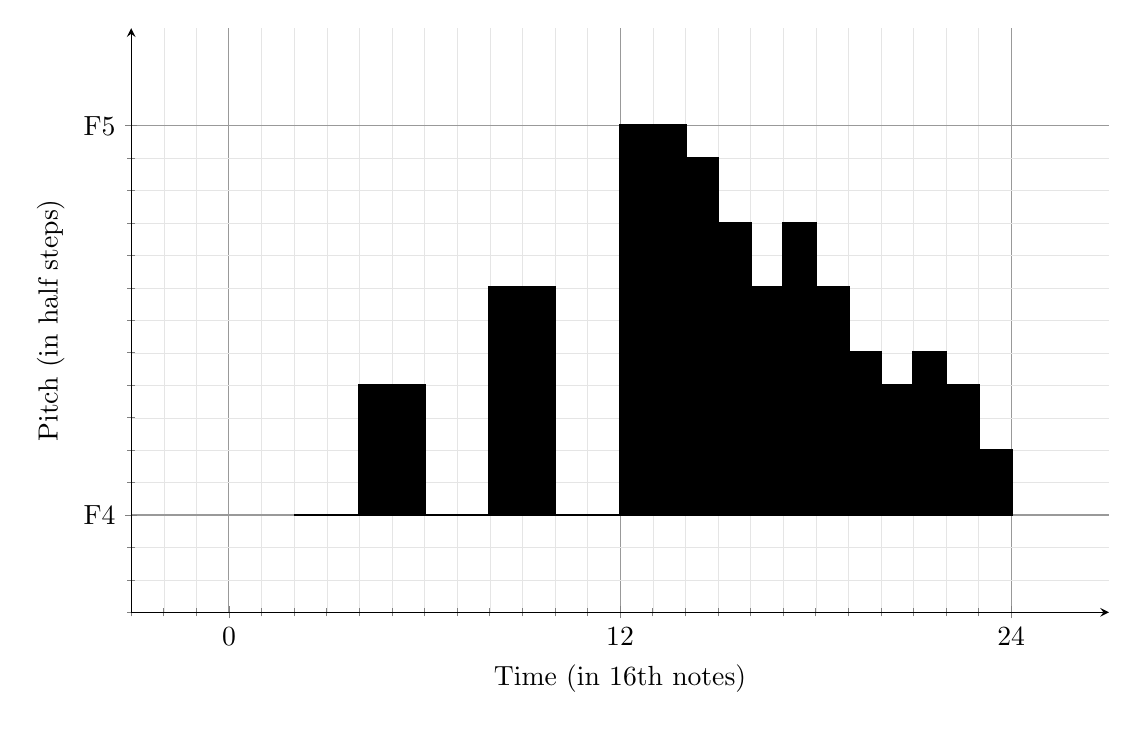
\begin{tikzpicture}
  \begin{axis}
    [
	ylabel= Pitch (in half steps),
	xlabel= Time (in 16th notes),
	grid=both,
	ytick distance=12,
	xtick distance=12,
	% number of ticks in between grids, 9 ticks = 10 cells
	minor tick num=11,
	% define regular grid style with line width and color
	grid style={line width=.1pt, draw=black!10},
	% define major grid style with line width and color
	major grid style={line width=.4pt,draw=black!40},
	axis y line=left,
	axis x line=bottom,
	enlargelimits=false,
	% define width and height
	ymin=-3,
	ymax=15,
	xmin=-3,
	xmax=27,
	yticklabels={0, F4, F5},
	width=14cm, height=9cm
    ];
        \addplot [
        const plot,
	fill=black,
        draw=black,
	line width=1pt,
    ] coordinates {
        (2,0)
        (4,4)
        (6,0)
        (8,7)
        (10,0)
        (12,12)
        (14,11)
        (15,9)
        (16,7)
        (17,9)
        (18,7)
        (19,5)
        (20,4)
        (21,5)
        (22,4)
        (23,2)
        (24,0)
	}
	\closedcycle
	;
  \end{axis}
\end{tikzpicture}

\hspace*{0.9cm}\begin{lilypond}
	\language "english"
	\score {
		\new Staff {
			\omit Staff.BarLine
			\time 3/4
			\relative c' {
				r8 f-. a-. f-. c'-. f,-.
				f' e16 d c d c bf a bf a g
			}
		}
		\layout {
			\context {
				\Score
				proportionalNotationDuration = #(ly:make-moment 3/45)
			}
		}
	}
\end{lilypond}

\vspace*{-1ex}
\begin{center}
	\small{Barlines omitted to emphasize graph correlation}
\end{center}


\say{\say{Musical motion}, when projected into spatial configuration,}
Schillinger writes in Book XI, \say{possesses characteristics similar to that
of motion, action, growth, or other eventual processes. It particularly
resembles mechanical trajectories and projections of period phenomena, i.e.,
processes which are characterizerd by a high degree of regularity. As
mechanical trajectories are the inherent patterns of \say{musical motion},
music is capable of expressing everything which can be translated in a form of
motion.}

Schillinger's statement and the graph vivify one aspect of the relationship
between music and motion. It is quite evident that just as music may be
projected into a form of motion, so forms of motion may be converted into
music. The graph method of notation, i.e., the rectangular projection of music,
offers a device for securing congruence of quantity and structure. It offers a
new, vivid approach to such problems as variation through inversion, the
analysis of melody, the modernization and \say{antiquation} of music, the
variation of density in orchestration, the correlation of music and emotion,
and other phases of composition. To Schillinger, the problems of musical
components therefore presented these general aspects: 1) substituation of a
scientif method of recording a musical composition for inadequate systems of
notation; 2) modification of a musical work through variation of its geometric
properties; and 3) production of music from a system of number values
translated into geometric relations and thereafter into corresponding
components of the tonal art.

\section{Schillinger's Masterful Pedagogy}

One other aspect of Schillinger's method requires discussion. This relates to
the masterful pedagogy underlying his system. Discussion of the concepts basic
to it may give the impression that mastery of the material is difficult. This
is not ture. A student does not need to be aware of the influence of modern
mathematics and psychology on Schillinger's System in order to study his work.
Insofar as mathematics is concerned, he does not need to know more than
ordinary arithmetic. Many students studied with Schillinger by correspondence
without having more than a knowledge of elementary mathematics. Beginning
simply with an understanding of musical notation, students learned all phases
of composition, and completed the course equipped to compose in the larger
forms to orchestrate their work, and to compose directly for orchestral
groups.\footnote{Each branch of Schillinger's work contains novel ideas and
techniques as practical as they are daring. To be of use, a summary description
of these would require more space than this introductory essay will permit. The
reader is referred instead to the following materians in the text itself:
factorial continuity (I, 12), distributive powers (I, 12), displacement (II,
3), tonal expansion (II, 5), symmetrric tonics (II, 6), geometrical expansion
(III, 2), primary and secondary axes of melody (IV, 3), psychological dial (IV,
4), forms of trajectorial motion (IV, 5), symmetric harmony (V, 3 and 5),
theory of indirect modulation (V, 14), sigma (\Sigma) concept (V, 22 and VI,
2), melodization (VI, 1), harmonization of two-part counterpoint (VII, 11), and
strata harmony (Book IX). Roman numerals refer to the Books and Arabic numerals
refer to the Chapters.}

Schillinger's technique is one of building complex units from simple ones. In
pitch-scales, for example, he beins with a one-unit scale and proceeds
numerically to construc scales of a larger and larger number of units.
Mathematical theories of combination and permutation serve to reveal all of the
possible variations within certain scale patterns. From scales built on units
of the diatonic system, Schillinger proceeds to expanded scales, and finally to
scales based on symmetric intervals, a type unknown in traditional theory. By
the time the student has concluded his study of Book II, he has become aware of
all the scales which may be built on the 12 semitones of the equal temperament
system. The possibilities revealed by mathematical analysis are correlated with
the practices of different composers, for Schillinger had an encyclopedic
knowledge of musical usage and history. Copious illustration, including
original compositions produced by his techniques, vivifies every step of the
presentation.

Similar comprehensiveness and exhaustiveness marks the other phases of the
Schillinger System. Previous theorists had systematized and classified certain
areas of the tonal art.\footnote{In his book on \textit(Harmony) for example,
Walter Piston describes his purpose as follows: \say{The aim of this book is to
present as concisely as possible the harmonic common practice of composers of
the eighteenth and nineteenth centuries. Rules are announced as observations
reported, without attempt at their justification on \ae sthetic grounds or as
laws of nature.}} It is Schillinger's achievement---through the methods of
mathematics---that he systematizes, classifies and analyzes all the resources
of the tonal art. This is not to imply that music theory stops with
Schillinger. Rather it suggests that he has opened the door to the most
exacting and the most scientific explorations of the art. As Nicolas Slonimsky
has phrased it, Schillinger has done for music what Meneleyeff did for
chemistry: he has provided an exhaustive periodic chart of all its elements
making possible the discovery of those that are not now known.

\section{Summary of Theoretical Foundations}

By way of summary, the theoretical foundations of the Schillinger System may be described as follows. Viewing music as a space-time entity capable of graphic projection into space, Schillinger arrived at these fundamental ideas:

\begin{enumerate}
	\item That music is determined as a logical system in the Cartesian or Einsteinian manner, i.e., that it consists of a system of correlated variables.
	\item The \ae sthetic qualities of music may be analyzed into the geometric relation of its components: rhythm, melody, harmony.
	\item Variation may be achieved through modification of the inherent geometric relations.
	\item Music may be composed by taking a system of number values, transforming them into geometric relations, and thereafter into corresponding components of rhythm, melody and harmony.
	\item Just as the understanding of natural and biological forms requires an understanding of the laws of their growth---i.e., the forms of regularity and evolution, so an insight into music necessitates discovery of the patterns of regularity and evolution. This is what rhythm is.
	\item Musical patterns, viewed in teh universe of physical, biological and \ae sthetic objects, are only special cases of the general scheme of pattern-making.
	\item Schemes of pattern-making take their origin in natural and biological objects---the ratios of curvature of celestial trajectories; the formation of crystals; the division and multiplication of cells in growing things etc. When they are analyzed quantitatively, such patterns yield various number series.
	\item These number series or quantities projected into music excite the same cerebral centers as were stimulated by animate beauty.
	\item Thus, every great work of art, every great musical composition, realizes a certain mathematical logic. The creations of the non-mathematical musician involve such logic regardless of whether he is conscious of it or not. The \ae sthetic harmony embodied in all great musical compositions may be discovered through the application of mathematical techniques of analysis.
\end{enumerate}

In terms of the history of music and art, Schillinger has summarized his basic ideas as follows:

\begin{enumerate}
	\item Nature produces physical phenomena which reveal an \ae sthetic harmony to us; this harmony is due to periodic and combinatory processes; \ae sthetic realities embody mathematical logic.
	\item Man recreates \ae sthetic realities by reproducing the appearance of the physical realities through his own body or through a material at his command; this process involves mathematical logic regardless of whether the artist is conscious of it or not. Imitating nature in an artistic medium, the artist achieves the laws of mathematical logic through his sensuous experience. This is the intuitive period of art creation.
	\item Becoming more and more conscious int eh course of his evolution,
man begins to produce directly from the laws themselves. With the development
of the technique of handling the materials of the art medium (special
components) as well as rhythm of the composition as a whole (general
components: space, time), man is enabled to select the desired product and the
machine does the rest; this is the period of rational art creation. Thus the
evolution of art falls into a closed system. An \ae sthetic reality may be
either a natural product, a product of human creative intuition, or a product
of composition, realized through computation by mathematical logic.
\end{enumerate}

These ideas are developed in Schillinger's masterwork \textit{Mathematical
Basis of the Arts},\footnote{To be published shortly (according to this
footnote from 1945)} a work of world-shaking importance and revolutionary
implications in the field of \ae sthetics, in which he formulates the general
laws of mathematical logic underlying all art structures.

\section{Achievements of the Schillinger System}

Percy Scholes, the well-known writer on music, has recently said: \say{In every other age, the rules have been based more or less upon the music of the time\dots\ We are still teaching on the basis of these (tradition) rules, as every published harmony textbook shows---even Schoenberg's. Yet not merely the idiom but the very principles of the art have changed\dots\ }
